\documentclass[10pt]{article}
\usepackage{latexsym}
\usepackage{natbib}
\usepackage{graphicx}
\usepackage{caption}
\usepackage{subcaption}
\usepackage{listings}
\usepackage{amsmath}

\title{Homework 2: Independent Component Analysis}
\author{Name: Shun Zhang\\
Email address: \texttt{jensen.zhang@utexas.edu}\\
EID: \texttt{sz4554}}
\date{}

\begin{document}
\maketitle

\section{Independent Component Analysis}

In this report, I applied Independent Component Analysis on Blind Source
Separation problem. Let $U$ be the orignal sources, $A$ be mixing
operation. Let $X = A \times U$. The goal is to find a matrix $W$ such that
$U = W \times X$, which recover the sources from the observations. 

I used the batch update method described on the webpage,
\begin{equation}
	\label{eq:dana}
	\Delta W = \eta (I + (1 - 2Z) Y^T)W
\end{equation}
This is slightly different from the update eqation proved in Ng's note,
\begin{equation}
	\Delta W = \eta ((1 - 2Z) X^T + (W^T)^{-1})
	\label{eq:ng}
\end{equation}
Equation~\ref{eq:dana} is more efficient, as there is no inverse of matrix.
I tried to derive Equation~\ref{eq:dana} from Equation~\ref{eq:ng},
\begin{align}
	\Delta W &= \eta ((1 - 2Z) X^T + (W^T)^{-1}) \\
	&= \eta ((1 - 2Z) X^T + (W^T)^{-1})W^T (W^T)^{-1} \\
	&= \eta ((1 - 2Z) X^T W^T + I)(W^T)^{-1} \\
	&= \eta ((1 - 2Z) (W X)^T + I)(W^T)^{-1} \\
	&= \eta ((1 - 2Z) Y^T + I)W (W^{-1})(W^T)^{-1} \\
	&= \eta ((1 - 2Z) Y^T + I)W (W^TW)^{-1}
	\label{eq:equiv}
\end{align}
So the different is the term, $W^TW$. If $W$ is othognal, then it's $W^TW =
I$. We know this is not a valid assumption. However, I used
Equation~\ref{eq:dana} in the experiments.

\section{Experiment}

\subsection{Experiments on Small Set}

\begin{figure}[h]
\centering
\begin{subfigure}{0.49\textwidth}
	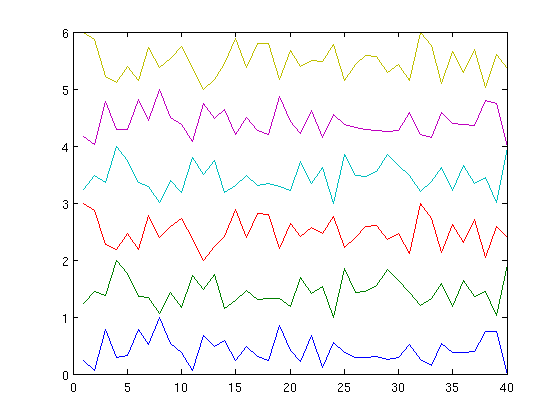
\includegraphics[width=\textwidth]{rep5.png}
\end{subfigure}
\begin{subfigure}{0.49\textwidth}
	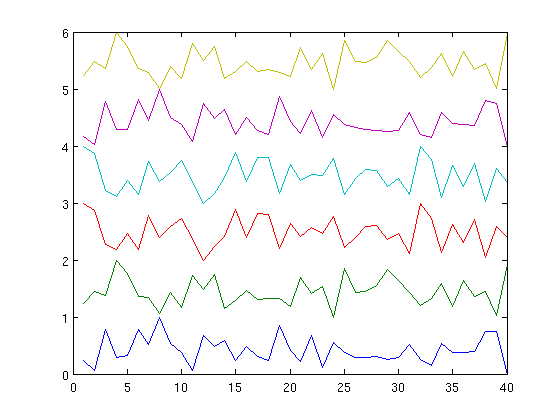
\includegraphics[width=\textwidth]{rep6.png}
\end{subfigure}
\caption{The bottom 3 lines are original signals from
\texttt{icaTest.mat}. The top 3 lines are reconstructed signals with $\eta
= 0.01$ and 1000000 iterations. Two independent experiments are shown.}
\label{fig:rep}
\end{figure}

\begin{table}
\centering
\begin{tabular}{ | l l l l | }
\hline
& Recon. 1& Recon. 2& Recon. 3\\
Source 1&-0.4900& \textbf{0.9905}& -0.4248\\
Source 2&\textbf{0.9918}& -0.3957& -0.5454\\
Source 3&-0.4829& -0.5073& \textbf{0.9924}\\
\hline
\end{tabular}
\caption{Linear correlation between source and reconstructed signals, for
the left figure in Figure~\ref{fig:rep}. The maximum correlation is
highlighted.}
\label{tbl:corr1}
\end{table}

\begin{table}
\centering
\begin{tabular}{ | l l l l | }
\hline
& Recon. 1& Recon. 2& Recon. 3\\
Source 1&-0.4248& \textbf{0.9905}&-0.4900\\
Source 2&-0.5454&-0.3957& \textbf{0.9918}\\
Source 3&\textbf{0.9924}&-0.5073&-0.4829\\
\hline
\end{tabular}
\caption{Linear correlation between source and reconstructed signals, for
the right figure in Figure~\ref{fig:rep}. The maximum correlation is
highlighted.}
\label{tbl:corr2}
\end{table}

The results are scaled into $[0, 1]$ interval. This experiment is repeated
twice.  The results are in shown in Figure~\ref{fig:rep}. The result can be
permutation of the original sources. Scaling is also possible (as the
results are scaled into $[0, 1]$, the signal could be flipped in this
case). The correlation between source and reconstructed signals are shown in
Table~\ref{tbl:corr1} and \ref{tbl:corr2}. They are highly correlated if
the correlavance is close to $1$ or $-1$. We can tell that, for the left figure,
the mapping is 0-4, 1-5, 2-3. While in the right one, the mapping is 0-5,
1-3, 2-4. This result can be verified visually. We can also observe that
the algorithm overall generate highly close signal, with has more than
$0.99$ correlavance with its source signal.

\begin{figure}
\centering
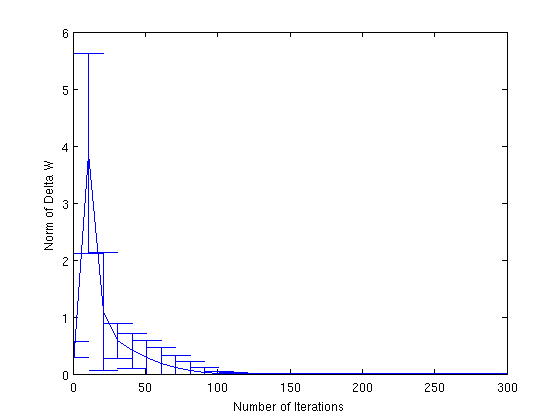
\includegraphics[width=.6\textwidth]{detW.png}
\caption{$\Delta W$ over number of iterations. Average of 5 runs. The
length of vertical bars is $\sigma$ assmuing Gaussian distribution of data
points at each iteration.}
\label{fig:detW}
\end{figure}

I also examine how progress is made in each iteration in the learning
process. As the algorithm uses gradient descent, the update on $W$ each
step, which is $\Delta W$, is useful. For the convenience of visualization,
I need the magtitude of this matrix. I use the largest singular value here,
which can be got using \texttt{norm} function when applied to a matrix in
Matlab.

The result is shown in Figure~\ref{fig:detW}. Not surprisingly, steps
become smaller after more iterations. The algorithm converges after $2
\times 10^5$ iterations.

\subsection{Experiments on Sound}

\begin{figure}
\centering
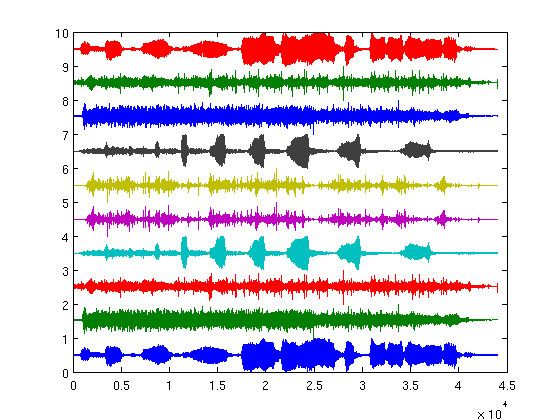
\includegraphics[width=.8\textwidth]{soundfull.png}
\caption{}
\label{fig:sound}
\end{figure}

\begin{table}
\centering
\begin{tabular}{ | l l l l l l | }
\hline
& Recon. 1& Recon. 2& Recon. 3& Recon. 4& Recon. 5\\
Source 1 &-0.0032& 0.0030&-0.0076&-0.0035& \textbf{1.0000}\\
Source 2 &-0.0014&-0.0003& \textbf{0.9999}&-0.0126& 0.0016\\
Source 3 &-0.0026&-0.0095& 0.0126& \textbf{0.9999}& 0.0007\\
Source 4 &0.0020& \textbf{0.9999}& 0.0083&-0.0102& 0.0041\\
Source 5 &\textbf{0.9999}& 0.0051& 0.0020& 0.0125&-0.0014\\
\hline
\end{tabular}
\caption{Linear correlation between source and reconstructed signals.}
\label{tbl:corrsf}
\end{table}

Result on sound are shown in Figure~\ref{fig:sound}. The correlation result
is shown in Table~\ref{tbl:corrs}. We can observe that the correlation is
smaller compared to that of experiment on small set.

\section{Discussion}

A batch version.

\section{Conclusion}

\end{document}
